% Đề kiểm tra cuối học kì 1 Toán 10 (chuyển đổi cấu trúc 2025: TN - Đúng/Sai - Trả lời ngắn)
% Tổng: 32 câu (26 Trắc nghiệm 4 PA, 3 Đúng/Sai, 3 Trả lời ngắn)

%%%%%%%%%%%%%%%% TRẮC NGHIỆM 4 PHƯƠNG ÁN %%%%%%%%%%%%%%%%

\begin{ex}%[0H9N2-1]
% nguon: Đề kiểm tra HK1 Toán 10 – Câu 1
	Trong mặt phẳng $Oxy$, cho vectơ $\vec{a}=(-6;8)$. Độ dài $\vec{a}$ là
	\choice
		{$|\vec{a}|=14$}
		{$|\vec{a}|=2$}
		{$|\vec{a}|=100$}
		{\True $|\vec{a}|=10$}
	\loigiai{
		Ta có $|\vec{a}|=\sqrt{(-6)^2+8^2}=\sqrt{36+64}=10$.
	}
\end{ex}

\begin{ex}%[0H4N1-2]
% nguon: Đề kiểm tra HK1 Toán 10 – Câu 2
	Cho góc $\alpha$ ($0^\circ \le \alpha \le 180^\circ$). Khẳng định nào đúng?
	\choice
		{\True $\sin(180^\circ-\alpha)=\sin\alpha$}
		{$\cos(180^\circ-\alpha)=\cos\alpha$}
		{$\tan(180^\circ-\alpha)=\tan\alpha$}
		{$\cot(180^\circ-\alpha)=\cot\alpha$}
	\loigiai{
		Theo tính chất hai góc bù nhau, ta có $\sin(180^\circ-\alpha)=\sin\alpha$.
	}
\end{ex}

\begin{ex}%[0D2N1-1]
% nguon: Đề kiểm tra HK1 Toán 10 – Câu 3
	Nghiệm của bất phương trình $2x+3y>5$ là
	\choice
		{$(1;-3)$}
		{$(2;-1)$}
		{\True $(2;5)$}
		{$(-2;-7)$}
	\loigiai{
		Thay $(2;5)$ vào bất phương trình ta được $2\cdot 2+3\cdot 5=19>5$ (đúng).
	}
\end{ex}

\begin{ex}%[0H9N2-1]
% nguon: Đề kiểm tra HK1 Toán 10 – Câu 4
	Trong mặt phẳng $Oxy$, cho hai vectơ $\vec{a}=(2;3)$ và $\vec{b}=(-1;4)$. Tích $\vec{a}\cdot\vec{b}$ là
	\choice
		{$\vec{a}\cdot\vec{b}=12$}
		{\True $\vec{a}\cdot\vec{b}=10$}
		{$\vec{a}\cdot\vec{b}=-10$}
		{$\vec{a}\cdot\vec{b}=-12$}
	\loigiai{
		Ta có $\vec{a}\cdot\vec{b}=2\cdot(-1)+3\cdot 4=-2+12=10$.
	}
\end{ex}

\begin{ex}%[0D1H2-2]
% nguon: Đề kiểm tra HK1 Toán 10 – Câu 5
	Cho tập hợp $M=\{x;y;z;t;k\}$. Số tập con có hai phần tử của $M$ là
	\choice
		{\True $10$ tập hợp}
		{$12$ tập hợp}
		{$24$ tập hợp}
		{$6$ tập hợp}
	\loigiai{
		Tập hợp $M$ có $5$ phần tử. Số tập con có $2$ phần tử của $M$ là $\mathrm{C}_5^2=10$ tập hợp.
	}
\end{ex}

\begin{ex}%[0D2N2-1]
% nguon: Đề kiểm tra HK1 Toán 10 – Câu 6
	Nghiệm của hệ bất phương trình $\heva{&2x-y\ge 1\\&x+y\le 4}$ là
	\choice
		{$(0;0)$}
		{\True $(2;-1)$}
		{$(1;5)$}
		{$(4;2)$}
	\loigiai{
		Thay $(2;-1)$ vào hệ bất phương trình ta được $\heva{&2\cdot 2-(-1)=5\ge 1\\&2+(-1)=1\le 4}$ (đúng).
	}
\end{ex}

\begin{ex}%[0H9N1-3]
% nguon: Đề kiểm tra HK1 Toán 10 – Câu 7
	Trong mặt phẳng $Oxy$, cho $\vec{v}=-3\vec{i}+7\vec{j}$. Tọa độ của vectơ $\vec{v}$ là
	\choice
		{\True $(-3;7)$}
		{$(3;-7)$}
		{$(7;-3)$}
		{$(-7;3)$}
	\loigiai{
		Vì $\vec{v}=-3\vec{i}+7\vec{j}$ nên tọa độ của vectơ $\vec{v}$ là $(-3;7)$.
	}
\end{ex}

\begin{ex}%[0D2N1-2]
% nguon: Đề kiểm tra HK1 Toán 10 – Câu 8
	Miền nghiệm của bất phương trình $3x-5y\le 8$ là
	\choice
		{\True Nửa mặt phẳng bờ là đường thẳng $d\colon 3x-5y=8$ chứa điểm $M(1;1)$ (kể cả bờ)}
		{Nửa mặt phẳng bờ là đường thẳng $d\colon 3x-5y=8$ không chứa điểm $M(1;1)$ (kể cả bờ)}
		{Nửa mặt phẳng bờ là đường thẳng $d\colon 3x-5y=8$ chứa điểm $M(1;1)$ (không kể bờ)}
		{Nửa mặt phẳng bờ là đường thẳng $d\colon 3x-5y=8$ không chứa điểm $M(1;1)$ (không kể bờ)}
	\loigiai{
		Thay tọa độ điểm $M(1;1)$ vào bất phương trình ta có $3\cdot 1-5\cdot 1=-2\le 8$ (đúng).\\
		Vì bất phương trình có dấu $\le$ nên miền nghiệm là nửa mặt phẳng bờ $d\colon 3x-5y=8$ chứa điểm $M(1;1)$ (kể cả bờ).
	}
\end{ex}

\begin{ex}%[0H4H2-2]
% nguon: Đề kiểm tra HK1 Toán 10 – Câu 9
	Cho tam giác $MNP$ có $MN=7\text{ cm}$, $NP=8\text{ cm}$, $MP=9\text{ cm}$. Diện tích tam giác $MNP$ là
	\choice
		{$5\sqrt{12}\text{ cm}^2$}
		{$7\sqrt{3}\text{ cm}^2$}
		{$3\sqrt{7}\text{ cm}^2$}
		{\True $12\sqrt{5}\text{ cm}^2$}
	\loigiai{
		Nửa chu vi tam giác $MNP$ là $p=\dfrac{7+8+9}{2}=12\text{ cm}$.\\
		Theo công thức Heron, diện tích tam giác $MNP$ là
		$S=\sqrt{12(12-7)(12-8)(12-9)}=\sqrt{12\cdot 5\cdot 4\cdot 3}=12\sqrt{5}\text{ cm}^2$.
	}
\end{ex}

\begin{ex}%[0D2N1-3]
% nguon: Đề kiểm tra HK1 Toán 10 – Câu 10
	Một cửa hàng dành tối đa $500$ triệu đồng để nhập $x$ xe đạp điện và $y$ xe đạp. Biết mỗi chiếc xe đạp điện có giá $8$ triệu đồng, mỗi chiếc xe đạp có giá $2$ triệu đồng. Bất phương trình biểu thị mối liên hệ của $x$ và $y$ là
	\choice
		{$8x+2y<500$}
		{$8x+2y>500$}
		{\True $8x+2y\le 500$}
		{$8x+2y\ge 500$}
	\loigiai{
		Tổng số tiền nhập $x$ xe đạp điện và $y$ xe đạp là $8x+2y$ (triệu đồng).\\
		Vì cửa hàng dành tối đa $500$ triệu đồng nên $8x+2y\le 500$.
	}
\end{ex}

\begin{ex}%[0H5N4-1]
% nguon: Đề kiểm tra HK1 Toán 10 – Câu 11
	Cho tam giác đều $ABC$ có $AB=5$. Giá trị của $\overrightarrow{AB}\cdot\overrightarrow{AC}$ bằng
	\choice
		{$25$}
		{$25\sqrt{2}$}
		{$25\sqrt{3}$}
		{\True $12{,}5$}
	\loigiai{
		Ta có $\overrightarrow{AB}\cdot\overrightarrow{AC}=AB\cdot AC\cdot\cos\widehat{BAC}=5\cdot 5\cdot\cos 60^\circ=25\cdot\dfrac{1}{2}=12{,}5$.
	}
\end{ex}

\begin{ex}%[0H4H2-1]
% nguon: Đề kiểm tra HK1 Toán 10 – Câu 12
	Cho tam giác $ABC$ cân tại $A$, có $AB=3$ và $\widehat{A}=120^\circ$. Giá trị của $BC$ là
	\choice
		{$3$}
		{\True $3\sqrt{3}$}
		{$3\sqrt{2}$}
		{$2\sqrt{3}$}
	\loigiai{
		Vì tam giác $ABC$ cân tại $A$ nên $AC=AB=3$.\\
		Theo định lí côsin: $BC^2=AB^2+AC^2-2AB\cdot AC\cos A=3^2+3^2-2\cdot 3\cdot 3\cdot\left(-\dfrac{1}{2}\right)=27$.\\
		Suy ra $BC=3\sqrt{3}$.
	}
\end{ex}

\begin{ex}%[0H5H3-6]
% nguon: Đề kiểm tra HK1 Toán 10 – Câu 13
	Cho tam giác đều $ABC$ nội tiếp đường tròn tâm $O$ bán kính bằng $3$. Gọi $H$ là điểm nằm trên đường tròn $(O)$, độ dài vectơ $\overrightarrow{HA}+\overrightarrow{HB}+\overrightarrow{HC}$ bằng
	\choice
		{\True $9$}
		{$8$}
		{$12$}
		{$7$}
	\loigiai{
		Vì tam giác $ABC$ đều nên tâm đường tròn ngoại tiếp $O$ trùng với trọng tâm của tam giác.\\
		Do đó $\overrightarrow{HA}+\overrightarrow{HB}+\overrightarrow{HC}=3\overrightarrow{HO}$.\\
		Suy ra $\left|\overrightarrow{HA}+\overrightarrow{HB}+\overrightarrow{HC}\right|=3HO=3\cdot 3=9$.
	}
\end{ex}

\begin{ex}%[0H5H4-1]
% nguon: Đề kiểm tra HK1 Toán 10 – Câu 14
	Cho tam giác $ABC$ vuông tại $A$, có $\widehat{C}=30^\circ$. Giá trị của $\cos\left(\overrightarrow{AB},\overrightarrow{BC}\right)$ là
	\choice
		{$\dfrac{1}{2}$}
		{\True $-\dfrac{1}{2}$}
		{$\dfrac{\sqrt{3}}{2}$}
		{$-\dfrac{\sqrt{3}}{2}$}
	\loigiai{
		Tam giác $ABC$ vuông tại $A$ có $\widehat{C}=30^\circ$ nên $\widehat{B}=60^\circ$.\\
		Ta có $\left(\overrightarrow{AB},\overrightarrow{BC}\right)=180^\circ-\widehat{B}=120^\circ$, suy ra $\cos\left(\overrightarrow{AB},\overrightarrow{BC}\right)=\cos 120^\circ=-\dfrac{1}{2}$.
	}
\end{ex}

\begin{ex}%[0D1H2-1]
% nguon: Đề kiểm tra HK1 Toán 10 – Câu 15
	Cho tập hợp $A=\{x\in\mathbb{Z}\mid 4\le x^2\le 17\}$. Tập hợp $A$ được viết dưới dạng liệt kê các phần tử là
	\choice
		{$A=\{2;3;4\}$}
		{$A=\{-4;-3;3;4\}$}
		{$A=\{-2;-3;-4;2;3\}$}
		{\True $A=\{-4;-3;-2;2;3;4\}$}
	\loigiai{
		Ta có $4\le x^2\le 17\Leftrightarrow 2\le |x|\le \sqrt{17}\approx 4{,}12$.\\
		Vì $x\in\mathbb{Z}$ nên $x\in\{-4;-3;-2;2;3;4\}$.
	}
\end{ex}

\begin{ex}%[0H4H1-3]
% nguon: Đề kiểm tra HK1 Toán 10 – Câu 16
	Biểu thức $P=(\sin a+\cos a)^2-2\sin a\cos a+\cot^2 a$ rút gọn được
	\choice
		{$P=\dfrac{1}{\cos^2 a}$}
		{$P=\tan^2 a$}
		{\True $P=\dfrac{1}{\sin^2 a}$}
		{$P=\cot^2 a$}
	\loigiai{
		Ta có $P=\sin^2 a+2\sin a\cos a+\cos^2 a-2\sin a\cos a+\cot^2 a=1+\cot^2 a=\dfrac{1}{\sin^2 a}$.
	}
\end{ex}

\begin{ex}%[0D6N1-3]
% nguon: Đề kiểm tra HK1 Toán 10 – Câu 17
	Trong một cuộc điều tra dân số, người ta báo cáo số dân của tỉnh A là $1\,435\,700\pm 200$ người. Số quy tròn số dân của tỉnh A đến hàng nghìn là
	\choice
		{$1\,435\,000$ người}
		{$1\,430\,000$ người}
		{\True $1\,436\,000$ người}
		{$1\,500\,000$ người}
	\loigiai{
		Chữ số hàng nghìn của $1\,435\,700$ là $5$, chữ số đứng ngay sau nó là $7\ge 5$ nên số quy tròn đến hàng nghìn là $1\,436\,000$ người.
	}
\end{ex}

\begin{ex}%[0D1N3-1]
% nguon: Đề kiểm tra HK1 Toán 10 – Câu 18
	Cho hai tập hợp $A=\{0;1;2;3;4;5\}$ và $B=\{-2;-1;0;1\}$. Tập hợp $A\cap B$ là
	\choice
		{$A\cap B=\{0;1;2;3;4;5\}$}
		{$A\cap B=\{-2;-1;0;1;2\}$}
		{\True $A\cap B=\{0;1\}$}
		{$A\cap B=\{-2;-1;0;1;2;3;4;5\}$}
	\loigiai{
		Các phần tử chung của hai tập hợp $A$ và $B$ là $0$ và $1$, do đó $A\cap B=\{0;1\}$.
	}
\end{ex}

\begin{ex}%[0D1N3-3]
% nguon: Đề kiểm tra HK1 Toán 10 – Câu 19
	Cho hai tập hợp $M=[3;7]$ và $N=[5;11)$. Tập hợp $M\cup N$ là
	\choice
		{$[3;5]$}
		{\True $[3;11)$}
		{$[3;11]$}
		{$[7;11]$}
	\loigiai{
		Ta có $M\cup N=[3;7]\cup [5;11)=[3;11)$.
	}
\end{ex}

\begin{ex}%[0H4H1-2]
% nguon: Đề kiểm tra HK1 Toán 10 – Câu 20
	Cho $\alpha$ ($90^\circ\le \alpha\le 180^\circ$) thỏa mãn $\sin\alpha=\dfrac{1}{2}$. Giá trị của $\cos\alpha$ là
	\choice
		{$\dfrac{\sqrt{3}}{2}$}
		{$\dfrac{3}{4}$}
		{\True $-\dfrac{\sqrt{3}}{2}$}
		{$-\dfrac{3}{4}$}
	\loigiai{
		Vì $90^\circ\le \alpha\le 180^\circ$ nên $\cos\alpha\le 0$.\\
		Ta có $\cos\alpha=-\sqrt{1-\sin^2\alpha}=-\sqrt{1-\dfrac{1}{4}}=-\dfrac{\sqrt{3}}{2}$.
	}
\end{ex}

\begin{ex}%[0H4H2-2]
% nguon: Đề kiểm tra HK1 Toán 10 – Câu 21
	Tam giác $ABC$ có $\widehat{B}+\widehat{C}=120^\circ$, $AC=10$, $AB=6$. Diện tích tam giác $ABC$ là
	\choice
		{\True $15\sqrt{3}$}
		{$13\sqrt{5}$}
		{$15\sqrt{5}$}
		{$30\sqrt{3}$}
	\loigiai{
		Ta có $\widehat{A}=180^\circ-(\widehat{B}+\widehat{C})=60^\circ$.\\
		Diện tích tam giác $ABC$ là $S=\dfrac{1}{2}AB\cdot AC\cdot\sin A=\dfrac{1}{2}\cdot 6\cdot 10\cdot\dfrac{\sqrt{3}}{2}=15\sqrt{3}$.
	}
\end{ex}

\begin{ex}%[0H4H1-2]
% nguon: Đề kiểm tra HK1 Toán 10 – Câu 22
	Giá trị của biểu thức $8\sin^4 45^\circ+\sqrt{3}\cot^3 150^\circ-2\tan 120^\circ$ là
	\choice
		{$2\sqrt{3}+1$}
		{$2$}
		{\True $2\sqrt{3}-7$}
		{$3$}
	\loigiai{
		Ta có $\sin 45^\circ=\dfrac{\sqrt{2}}{2}$, $\cot 150^\circ=-\sqrt{3}$, $\tan 120^\circ=-\sqrt{3}$.\\
		Thay vào biểu thức: $8\cdot\left(\dfrac{\sqrt{2}}{2}\right)^4+\sqrt{3}\cdot(-\sqrt{3})^3-2\cdot(-\sqrt{3})=8\cdot\dfrac{1}{4}-9+2\sqrt{3}=2\sqrt{3}-7$.
	}
\end{ex}

\begin{ex}%[0H5H2-2]
% nguon: Đề kiểm tra HK1 Toán 10 – Câu 23
	Cho hình bình hành $ABCD$. Gọi $M,N$ lần lượt là trung điểm của $AD,BC$. Khẳng định nào sai?
	\choice
		{$\overrightarrow{AD}+\overrightarrow{MB}+\overrightarrow{NA}=\vec{0}$}
		{$\overrightarrow{CD}-\overrightarrow{CA}+\overrightarrow{CB}=\vec{0}$}
		{$\overrightarrow{CD}-\overrightarrow{ND}+\overrightarrow{AM}=\vec{0}$}
		{\True $\overrightarrow{AB}+\overrightarrow{BM}+\overrightarrow{NC}=\vec{0}$}
	\loigiai{
		Ta có $\overrightarrow{AB}+\overrightarrow{BM}+\overrightarrow{NC}=\overrightarrow{AM}+\overrightarrow{NC}$.\\
		Vì $ABCD$ là hình bình hành và $M,N$ lần lượt là trung điểm của $AD,BC$ nên $\overrightarrow{AM}=\overrightarrow{NC}\ne \vec{0}$.\\
		Suy ra $\overrightarrow{AB}+\overrightarrow{BM}+\overrightarrow{NC}=2\overrightarrow{NC}\ne\vec{0}$.
	}
\end{ex}

\begin{ex}%[0H4N2-1]
% nguon: Đề kiểm tra HK1 Toán 10 – Câu 24
	Cho tam giác $ABC$ có $BC=5$ và $\widehat{A}=30^\circ$. Bán kính đường tròn ngoại tiếp tam giác $ABC$ là
	\choice
		{\True $5$}
		{$10$}
		{$5\sqrt{3}$}
		{$10\sqrt{3}$}
	\loigiai{
		Theo định lí sin ta có $R=\dfrac{BC}{2\sin A}=\dfrac{5}{2\sin 30^\circ}=\dfrac{5}{2\cdot\tfrac{1}{2}}=5$.
	}
\end{ex}

\begin{ex}%[0H4V3-2]
% nguon: Đề kiểm tra HK1 Toán 10 – Câu 25
	\immini{
		Một người quan sát đứng cách một cái tháp $20\text{ m}$, nhìn thẳng cái tháp dưới một góc $55^\circ$ như hình vẽ (với $AD=20\text{ m}$, $\widehat{CAD}=45^\circ$, $\widehat{DAB}=10^\circ$ và $AD\perp BC$). Chiều cao của tháp là
		\choice
			{$20\text{ m}$}
			{\True $23{,}53\text{ m}$}
			{$20{,}53\text{ m}$}
			{$25{,}35\text{ m}$}
	}{
		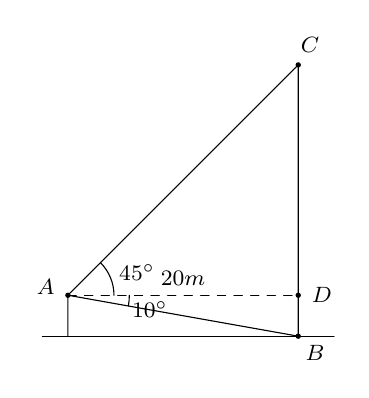
\begin{tikzpicture}[scale=0.65, font=\footnotesize, line join=round, line cap=round]
			\coordinate (A) at (0,0.8);
			\coordinate (D) at (4.5,0.8);
			\coordinate (C) at (4.5,5.3);
			\coordinate (B) at (4.5,0);
			\coordinate (H) at (0,0);
			\draw (-0.5,0)--(5.2,0);
			\draw (A)--(H) (A)--(C)--(B)--(A);
			\draw[dashed] (A)--(D) node[midway,above]{$20\text{ m}$};
			\draw (A)++(0:0.9) arc (0:45:0.9);
			\node at (1.35,1.25) {$45^\circ$};
			\draw (A)++(-10:1.2) arc (-10:0:1.2);
			\node at (1.6,0.52) {$10^\circ$};
			\foreach \p/\g in {A/160, C/60, D/0, B/-45}
				\fill (\p) circle (1.5pt) node[shift={(\g:3mm)}]{$\p$};
		\end{tikzpicture}
	}
	\loigiai{
		Xét hai tam giác vuông $ADC$ và $ADB$ (vuông tại $D$), ta có:\\
		$CD=AD\cdot\tan 45^\circ=20\cdot 1=20\text{ m}$;\\
		$BD=AD\cdot\tan 10^\circ\approx 20\cdot 0{,}1763\approx 3{,}53\text{ m}$.\\
		Vậy chiều cao của tháp là $BC=CD+BD\approx 20+3{,}53=23{,}53\text{ m}$.
	}
\end{ex}

\begin{ex}%[0H5H3-2]
% nguon: Đề kiểm tra HK1 Toán 10 – Câu 26
	Cho tam giác $ABC$ có trọng tâm là $G$ và $M$ là trung điểm của $BC$. Mệnh đề nào sai?
	\choice
		{$\overrightarrow{AG}=\dfrac{2}{3}\overrightarrow{AM}$}
		{$\overrightarrow{AB}+\overrightarrow{AC}=3\overrightarrow{AG}$}
		{$\overrightarrow{GA}=\overrightarrow{BG}+\overrightarrow{CG}$}
		{\True $\overrightarrow{GB}+\overrightarrow{GC}=\overrightarrow{GM}$}
	\loigiai{
		Vì $M$ là trung điểm của $BC$ nên $\overrightarrow{GB}+\overrightarrow{GC}=2\overrightarrow{GM}\ne\overrightarrow{GM}$.
	}
\end{ex}

%%%%%%%%%%%%%%%% ĐÚNG/SAI %%%%%%%%%%%%%%%%

\begin{ex}%[0D6H4-4]
% nguon: Đề kiểm tra HK1 Toán 10 – Câu 27-30
	Điểm thi môn Toán cuối học kì $1$ của lớp $10\text{A}$ được cho trong bảng sau:
	\begin{center}
		\begin{tabular}{|l|c|c|c|c|c|c|c|c|c|}
			\hline
			Điểm & $10$ & $9{,}5$ & $9$ & $8{,}5$ & $8$ & $7{,}5$ & $7$ & $6{,}5$ & $6$ \\
			\hline
			Số bạn & $4$ & $5$ & $7$ & $8$ & $5$ & $4$ & $2$ & $3$ & $2$ \\
			\hline
		\end{tabular}
	\end{center}
	Xét tính đúng sai của các khẳng định sau:
	\choiceTF
		{\True Giá trị trung bình của mẫu số liệu là $8{,}35$}
		{\True Mốt của mẫu số liệu trên là $8{,}5$}
		{Phương sai của mẫu số liệu (làm tròn đến hàng phần trăm) là $1{,}37$}
		{\True Độ lệch chuẩn của mẫu số liệu (làm tròn đến hàng phần trăm) là $1{,}11$}
	\loigiai{
		\begin{itemchoice}
			\itemch Đúng. Cỡ mẫu $n=4+5+7+8+5+4+2+3+2=40$.\\
			Giá trị trung bình là $\overline{x}=\dfrac{10\cdot 4+9{,}5\cdot 5+9\cdot 7+8{,}5\cdot 8+8\cdot 5+7{,}5\cdot 4+7\cdot 2+6{,}5\cdot 3+6\cdot 2}{40}=\dfrac{334}{40}=8{,}35$.
			\itemch Đúng. Giá trị có tần số lớn nhất (bằng $8$) là $8{,}5$ nên mốt $M_o=8{,}5$.
			\itemch Sai. Phương sai của mẫu số liệu là
			$s^2=\dfrac{1}{40}\left[4(10-8{,}35)^2+5(9{,}5-8{,}35)^2+\dots+2(6-8{,}35)^2\right]=1{,}2275\approx 1{,}23$.
			\itemch Đúng. Độ lệch chuẩn là $s=\sqrt{1{,}2275}\approx 1{,}11$.
		\end{itemchoice}
	}
\end{ex}

\begin{ex}%[0D2V2-3]
% nguon: Đề kiểm tra HK1 Toán 10 – Tự luận Câu 1
	Mẹ đi chợ mua $x$ con gà và $y$ con vịt ($x,y\in\mathbb{N}$). Biết rằng mỗi con gà giá $180$ nghìn đồng, mỗi con vịt giá $120$ nghìn đồng. Số tiền mẹ mua không quá $2$ triệu đồng và mua được nhiều hơn $13$ con. Xét tính đúng sai của các khẳng định sau:
	\choiceTF
		{\True Bất phương trình biểu thị điều kiện về số tiền mua là $9x+6y\le 100$}
		{Bất phương trình biểu thị điều kiện về tổng số con mua được là $x+y\ge 13$}
		{\True Mẹ có thể mua $5$ con gà và $9$ con vịt để thỏa mãn các điều kiện trên}
		{Số tiền ít nhất mẹ cần chi để thỏa mãn điều kiện bài toán là $1\,740$ nghìn đồng}
	\loigiai{
		\begin{itemchoice}
			\itemch Đúng. Tổng số tiền không quá $2\,000$ nghìn đồng nên $180x+120y\le 2000\Leftrightarrow 9x+6y\le 100$.
			\itemch Sai. Vì mẹ mua được nhiều hơn $13$ con nên $x+y>13$.
			\itemch Đúng. Với $x=5$, $y=9$ ta có $5+9=14>13$ và $180\cdot 5+120\cdot 9=1980\le 2000$ (thỏa mãn).
			\itemch Sai. Để chi ít tiền nhất mà vẫn mua nhiều hơn $13$ con (tối thiểu $14$ con), mẹ mua $0$ con gà và $14$ con vịt với số tiền $14\cdot 120=1\,680$ nghìn đồng.
		\end{itemchoice}
	}
\end{ex}

\begin{ex}%[0H5V4-4]
% nguon: Đề kiểm tra HK1 Toán 10 – Tự luận Câu 3
	Cho tam giác $ABC$ có $AB=AC=5\text{ cm}$ và $\widehat{BAC}=120^\circ$. Gọi $H$ là chân đường cao kẻ từ $A$ xuống $BC$, điểm $M$ thỏa mãn $\overrightarrow{MA}+3\overrightarrow{AC}=\vec{0}$ và điểm $N$ trên cạnh $BC$ sao cho $\overrightarrow{BN}=x\overrightarrow{BC}$. Xét tính đúng sai của các khẳng định sau:
	\choiceTF
		{\True $\overrightarrow{AB}\cdot\overrightarrow{CA}=12{,}5$}
		{\True Độ dài cạnh $BC$ bằng $5\sqrt{3}\text{ cm}$}
		{Độ dài đường cao $AH$ bằng $2{,}5\sqrt{3}\text{ cm}$}
		{\True Để $AN\perp BM$ thì $x=\dfrac{5}{12}$}
	\loigiai{
		\begin{itemchoice}
			\itemch Đúng. Ta có $\overrightarrow{AB}\cdot\overrightarrow{CA}=-\overrightarrow{AB}\cdot\overrightarrow{AC}=-5\cdot 5\cdot\cos 120^\circ=12{,}5$.
			\itemch Đúng. Theo định lí côsin: $BC=\sqrt{AB^2+AC^2-2AB\cdot AC\cos 120^\circ}=\sqrt{25+25+25}=5\sqrt{3}\text{ cm}$.
			\itemch Sai. Tam giác $ABC$ cân tại $A$ có $\widehat{A}=120^\circ$ nên $\widehat{B}=30^\circ$, suy ra $AH=AB\sin 30^\circ=5\cdot\dfrac{1}{2}=2{,}5\text{ cm}$.
			\itemch Đúng. Ta có $\overrightarrow{AM}=3\overrightarrow{AC}\Rightarrow \overrightarrow{BM}=3\overrightarrow{AC}-\overrightarrow{AB}$ và $\overrightarrow{AN}=(1-x)\overrightarrow{AB}+x\overrightarrow{AC}$.\\
			Do $AN\perp BM\Leftrightarrow \overrightarrow{AN}\cdot\overrightarrow{BM}=0\Leftrightarrow \left[(1-x)\overrightarrow{AB}+x\overrightarrow{AC}\right]\cdot\left(3\overrightarrow{AC}-\overrightarrow{AB}\right)=0$\\
			$\Leftrightarrow (3-4x)\overrightarrow{AB}\cdot\overrightarrow{AC}-(1-x)AB^2+3xAC^2=0$\\
			$\Leftrightarrow (3-4x)(-12{,}5)-25(1-x)+75x=0\Leftrightarrow 150x-62{,}5=0\Leftrightarrow x=\dfrac{5}{12}$.
		\end{itemchoice}
	}
\end{ex}

%%%%%%%%%%%%%%%% TRẢ LỜI NGẮN %%%%%%%%%%%%%%%%

\begin{bt}%[0H4V1-3]
% nguon: Đề kiểm tra HK1 Toán 10 – Tự luận Câu 2
	Tính giá trị của biểu thức $P=\sqrt{\sin^4 x+6\cos^2 x+3\cos^4 x}+\sqrt{\cos^4 x+6\sin^2 x+3\sin^4 x}$ (biết giá trị của $P$ không phụ thuộc vào $x$).
	\shortans{4}
	\loigiai{
		Ta có $\sin^4 x+6\cos^2 x+3\cos^4 x=(1-\cos^2 x)^2+6\cos^2 x+3\cos^4 x=1+4\cos^2 x+4\cos^4 x=(1+2\cos^2 x)^2$.\\
		Tương tự, $\cos^4 x+6\sin^2 x+3\sin^4 x=(1+2\sin^2 x)^2$.\\
		Vì $1+2\cos^2 x>0$ và $1+2\sin^2 x>0$ nên
		$P=(1+2\cos^2 x)+(1+2\sin^2 x)=2+2(\cos^2 x+\sin^2 x)=4$.
	}
\end{bt}

\begin{bt}%[0H4H2-2]
% nguon: Đề kiểm tra HK1 Toán 10 – Tự luận Câu 3b
	Cho tam giác $ABC$ có $AB=AC=5\text{ cm}$ và $\widehat{BAC}=120^\circ$. Tính độ dài đường cao $AH$ ($H\in BC$) theo đơn vị cm.
	\shortans{2,5}
	\loigiai{
		Tam giác $ABC$ cân tại $A$ có $\widehat{BAC}=120^\circ$ nên $\widehat{B}=30^\circ$.\\
		Trong tam giác vuông $AHB$, ta có $AH=AB\cdot\sin B=5\cdot\sin 30^\circ=2{,}5\text{ cm}$.
	}
\end{bt}

\begin{bt}%[0H5V4-4]
% nguon: Đề kiểm tra HK1 Toán 10 – Tự luận Câu 3c
	Cho tam giác $ABC$ có $AB=AC=5\text{ cm}$ và $\widehat{BAC}=120^\circ$. Gọi $M$ là điểm thỏa mãn $\overrightarrow{MA}+3\overrightarrow{AC}=\vec{0}$ và $N$ là điểm trên cạnh $BC$ sao cho $\overrightarrow{BN}=x\overrightarrow{BC}$. Tìm $x$ để $AN\perp BM$ (làm tròn kết quả đến hàng phần trăm).
	\shortans{0,42}
	\loigiai{
		Ta có $\overrightarrow{AB}\cdot\overrightarrow{AC}=5\cdot 5\cdot\cos 120^\circ=-12{,}5$.\\
		Từ giả thiết: $\overrightarrow{BM}=\overrightarrow{AM}-\overrightarrow{AB}=3\overrightarrow{AC}-\overrightarrow{AB}$ và $\overrightarrow{AN}=(1-x)\overrightarrow{AB}+x\overrightarrow{AC}$.\\
		Điều kiện $AN\perp BM\Leftrightarrow \overrightarrow{AN}\cdot\overrightarrow{BM}=0\Leftrightarrow (3-4x)\overrightarrow{AB}\cdot\overrightarrow{AC}-(1-x)AB^2+3xAC^2=0$\\
		$\Leftrightarrow (3-4x)(-12{,}5)-25(1-x)+75x=0\Leftrightarrow 150x=62{,}5\Leftrightarrow x=\dfrac{5}{12}\approx 0{,}42$.
	}
\end{bt}
